% https://habrahabr.ru/post/145523/
% http://fsweb.info/editors/latex/presentation.html
\documentclass[10pt]{beamer}
\usepackage[utf8]{inputenc}
\usepackage[T2A]{fontenc}
\usepackage[english, russian]{babel}
\usepackage{amsmath,amsfonts,amssymb}
\usepackage{graphicx}
%\usetheme{Singapore}
% \usetheme{Berlin}
% \usetheme{CambridgeUS}
\usetheme{CambridgeUS}

%\setbeamercolor{элемент}{bg=цвет1,fg=цвет2}. Здесь «элемент» — название элемента, чей цвет мы хотим изменить (например, «normal text» — обычный текст), «bg» — цвет фона, «fg» — цвет текста.
%\usebackgroundtemplate{\includegraphics[width=\paperwidth,height=\paperheight]{my_backgroung_picture.jpg}}

\addto\captionsrussian{\renewcommand{\figurename}{Рис.}}
\setbeamertemplate{caption}[numbered]

\RequirePackage{caption}
\DeclareCaptionLabelSeparator{defffis}{ -- }
\captionsetup{justification=centering,labelsep=defffis}

\newcommand{\MB}{\mathbf}
\newcounter{myexmpl}



\begin{document}


\title{Эргономика компьютерных игр}
\subtitle{презентация по курсу ``Человеко-компьютерное взаимодействие''}
\logo{
\includegraphics[width=0.15\textwidth]{res/img/titlePage/sfedu.png}}
\author{В.Э. Смирнов,
        Д.В. Сухоловский,
        В.С. Фоменко}
\institute{
  МИНОБРНАУКИ РОССИИ \\
  Федеральное государственное автономное образовательное учреждение   высшего образования \\
  <<ЮЖНЫЙ ФЕДЕРАЛЬНЫЙ УНИВЕРСИТЕТ>> \\
  Институт Компьютерных технологий и информационной безопасности \\
  Кафедра Математического обеспечения и применения ЭВМ
}
\date{\the\year~год}
\setbeamercovered{transparent}
% Если в нашей презентации используется последовательное высвечивание элементов, стоит сказать: \setbeamercovered{transparent}, чтобы неактивные элементы были хотя бы немного видны.

%\setbeamertemplate{navigation symbols}{}  %убрать панель навигации

%	\author{}
	%\title{}
	%\subtitle{}
	%\logo{}
	%\institute{}
	%\date{}
	%\subject{}
	%\setbeamercovered{transparent} % или dynamic
	%\setbeamertemplate{navigation symbols}{}


\begin{frame}[plain]
	%\maketitle
  \titlepage
\end{frame}

\begin{frame}
  \frametitle{Содержание}
  \tableofcontents
\end{frame}

%%%%%%%%%%%%%%%%%%%%%%%%%%%%%%%%%%%%%%%%%%%%%%%%%%%%%%%%%%%%%%%%%%%%%
\section{Введение}

% \subsection{Особенности СТУ}

%%%%%%%%%%%%%%%%%%%%%%%%%%  слайд 3 %%%%%%%%%%%%%%%%%%%%%%%%%%%%
\begin{frame}
  \frametitle{Введение}

  \begin{columns}[c]
  \column{0.5\textwidth}

  \begin{center}
    % 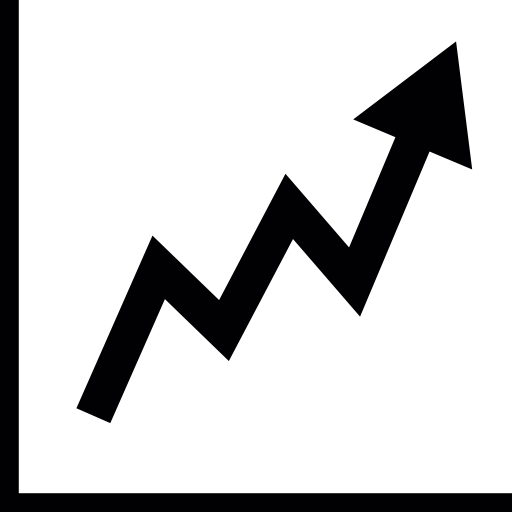
\includegraphics[width=0.8\textwidth]{res/img/improve.png}
    Улучшение
  \end{center}

  \column{0.5\textwidth}
  \begin{block}{}
    Разработка интерфейсов игровых программ предполагает не только решение сугубо утилитарных задач, связанных с обеспечением простоты и удобства управления игрой, но еще и создание у пользователя определенного эмоционального настроя.
  \end{block}
  \end{columns}
\end{frame}


%\hyphenation{-удовлетворения}
\begin{frame}
\frametitle{Введение}

\begin{columns}[c]
\column{0.5\textwidth}

\begin{center}
  % 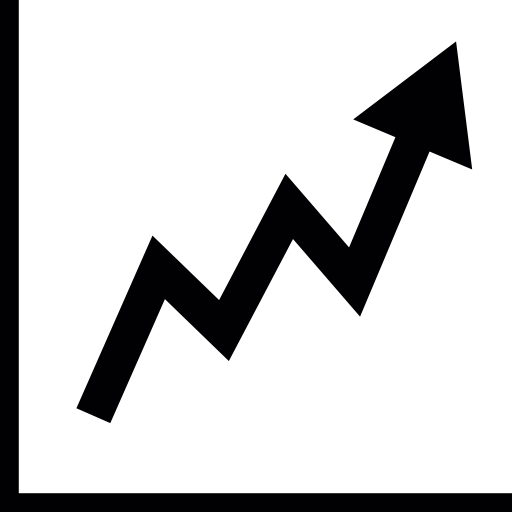
\includegraphics[width=0.8\textwidth]{res/img/improve.png}
  Улучшение
\end{center}

\column{0.5\textwidth}
\begin{block}{}
  Хорошая игра должна:
  \begin{itemize}
    \item увлекать и всецело затягивать;
    \item вызывать чувство эстетического  удовлетворения.
  \end{itemize}
\end{block}
\end{columns}
\end{frame}

\section{Факторы, влияющие на удовлетворение игрока}
\begin{frame}
\frametitle{Факторы, влияющие на удовлетворение игрока}

\begin{columns}[c]
\column{0.5\textwidth}

\begin{center}
  % 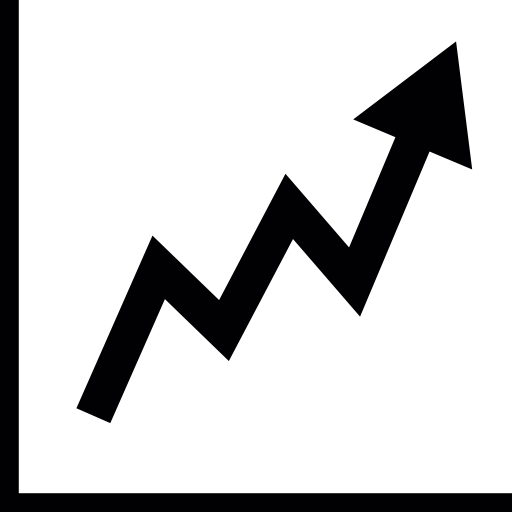
\includegraphics[width=0.8\textwidth]{res/img/improve.png}
  Улучшение
\end{center}

\column{0.5\textwidth}
\begin{block}{}

  \begin{itemize}
    \item Простота использования;
    \item Ритм игры;
    \item Степень трудности игры.
  \end{itemize}
\end{block}
\end{columns}
\end{frame}

\subsection{Простота использования}
\begin{frame}
\frametitle{Простота использования}

\begin{columns}[c]
\column{0.5\textwidth}

\begin{center}
  % 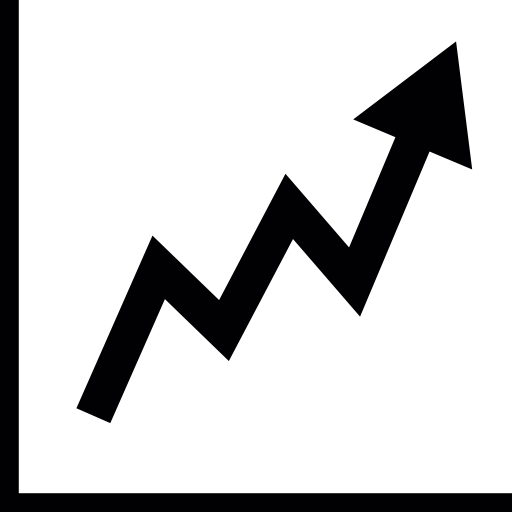
\includegraphics[width=0.8\textwidth]{res/img/improve.png}
  Улучшение
\end{center}

\column{0.5\textwidth}
\begin{block}{}

  \textbf{Начало игры} -- Меню, с помощью которого осуществляется запуск игры, следует уделять особое внимание. Разработчик должен быть уверенным в том, что:
  \begin{itemize}
    \item пользователь получил исчерпывающую информацию о возможностях игры;
    \item после ознакомления с меню пользователь может управлять игровым процессом без проблем.
  \end{itemize}

\end{block}
\end{columns}
\end{frame}

\begin{frame}
\frametitle{Простота использования}

\begin{columns}[c]
\column{0.5\textwidth}

\begin{center}
  % 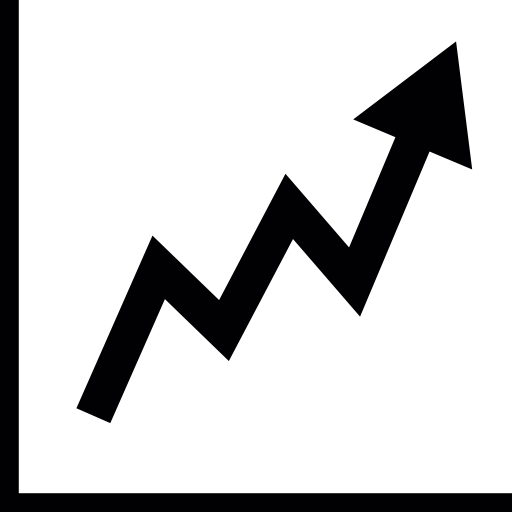
\includegraphics[width=0.8\textwidth]{res/img/improve.png}
  Улучшение
\end{center}

\column{0.5\textwidth}
\begin{block}{}

  \textbf{Обучающие уровни} -- Если игра включает обучающие уровни, то они должны быть органичной ее частью. Они должны отвечать следующим требованиям:
  \begin{itemize}
    \item не быть как слишком трудными, так и слишком легкими;
    \item после прохождения обучающих уровней у пользователя должно возникнуть желание продолжать игру.
  \end{itemize}

\end{block}
\end{columns}
\end{frame}

\begin{frame}
\frametitle{Простота использования}

\begin{columns}[c]
\column{0.5\textwidth}

\begin{center}
  % 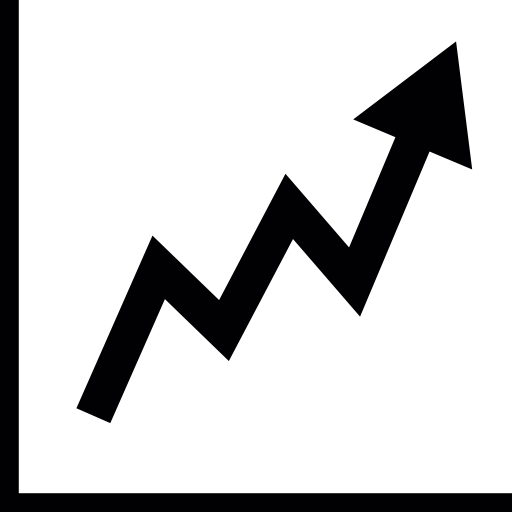
\includegraphics[width=0.8\textwidth]{res/img/improve.png}
  Улучшение
\end{center}

\column{0.5\textwidth}
\begin{block}{}

  \textbf{Игровой интерфейс} -- Его задачей является обеспечение обратной связи с пользователем, а также осуществление некоторых действий. К игровым интерфейсам применяются такие же требования, как и к интерфейсу любого ПО.

\end{block}
\end{columns}
\end{frame}

\begin{frame}
\frametitle{Простота использования}

\begin{columns}[c]
\column{0.5\textwidth}

\begin{center}
  % 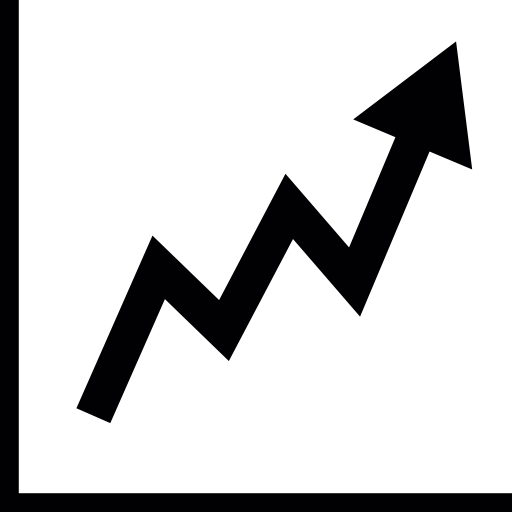
\includegraphics[width=0.8\textwidth]{res/img/improve.png}
  Улучшение
\end{center}

\column{0.5\textwidth}
\begin{block}{}

  \textbf{Управление игрой с помощью периферийных устройств} -- Управление любой периферией должно осуществляться <<на автомате>>. Выбор кнопок и их функции должны быть обусловлены исключительно удобством пользователя.

\end{block}
\end{columns}
\end{frame}

\begin{frame}
\frametitle{Рекомендации}

\begin{columns}[c]
\column{0.5\textwidth}

\begin{center}
  % 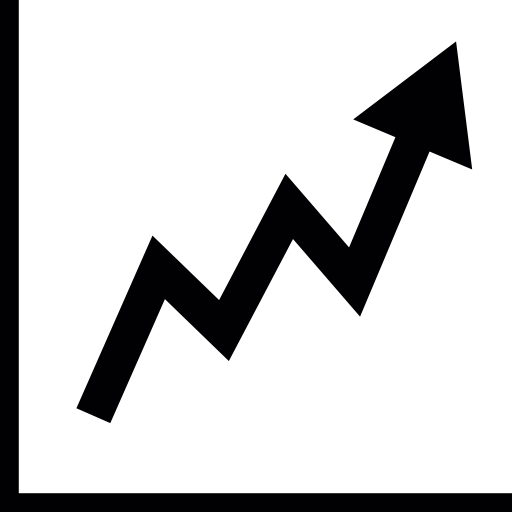
\includegraphics[width=0.8\textwidth]{res/img/improve.png}
  Улучшение
\end{center}

\column{0.5\textwidth}
\begin{block}{}

\begin{itemize}
  \item Избегайте продолжительных вступлений.
  \item Старайтесь как можно органичнее встраивать индикаторы в игровое окружение.
  \item Используйте модели повреждения или другие уникальные контекстуальные решения вместо индикаторов здоровья.
  \item Используйте простую контекстно зависимую систему управления вместо сложной и обширной.
\end{itemize}

\end{block}
\end{columns}
\end{frame}

\subsection{Ритм игры}
\begin{frame}
\frametitle{Ритм игры}

\begin{columns}[c]
\column{0.5\textwidth}

\begin{center}
  % 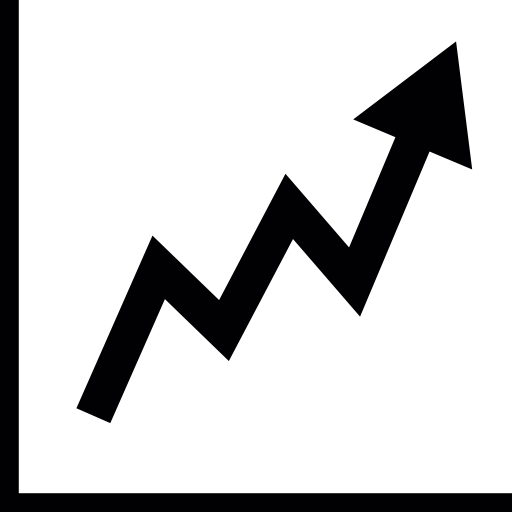
\includegraphics[width=0.8\textwidth]{res/img/improve.png}
  Улучшение
\end{center}

\column{0.5\textwidth}
\begin{block}{}
Ритм игры - это то что затягивает в игровой процесс. Прежде всего это:
\begin{itemize}
  \item интерактивность;
  \item сюжет.
\end{itemize}

\end{block}
\end{columns}
\end{frame}

\begin{frame}
\frametitle{Рекомендации}

\begin{columns}[c]
\column{0.5\textwidth}

\begin{center}
  % 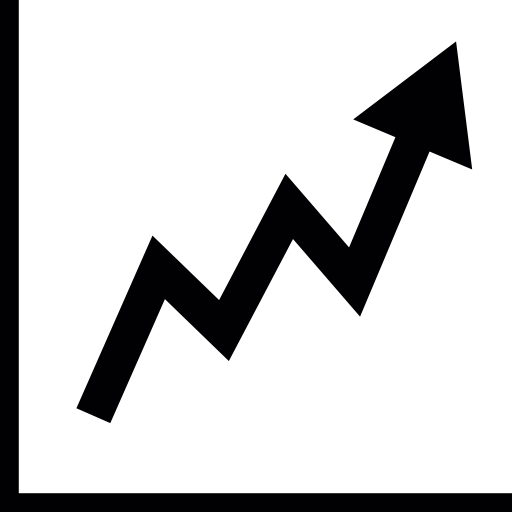
\includegraphics[width=0.8\textwidth]{res/img/improve.png}
  Улучшение
\end{center}

\column{0.5\textwidth}
\begin{block}{}

\begin{itemize}
  \item Больше исследований, меньше объяснений.
  \item Избегайте дополнительных предметов коллекций.
  \item Молчание может быть содержательней диалога.
  \item Заставляйте игрока ставить вопросы и не бойтесь оставлять их без ответа.
  \item Простой сюжет можно компенсировать, выдвинув на первый план процесс совершенствования игрока.
\end{itemize}

\end{block}
\end{columns}
\end{frame}

\subsection{Степень трудности игры}
\begin{frame}
\frametitle{Степень трудности игры}

\begin{columns}[c]
\column{0.5\textwidth}

\begin{center}
  % 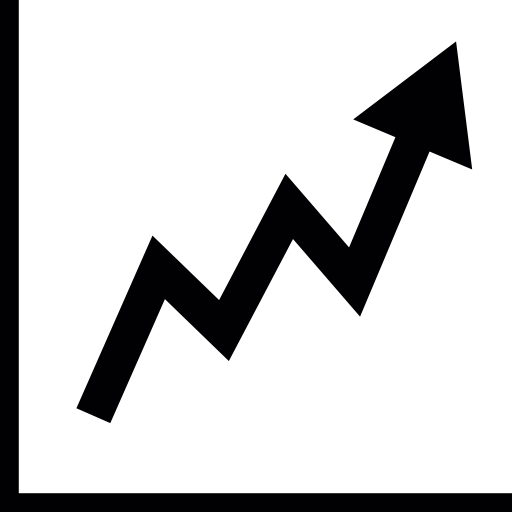
\includegraphics[width=0.8\textwidth]{res/img/improve.png}
  Улучшение
\end{center}

\column{0.5\textwidth}
\begin{block}{}

\begin{itemize}
  \item Сложность
  \item Тип задачи.
  \item Вознаграждение.
\end{itemize}

\end{block}
\end{columns}
\end{frame}




\end{document}
